\begin{figure}
	\centering
% Created by tikzDevice version 0.12.3.1 on 2022-09-20 11:16:37
% !TEX encoding = UTF-8 Unicode
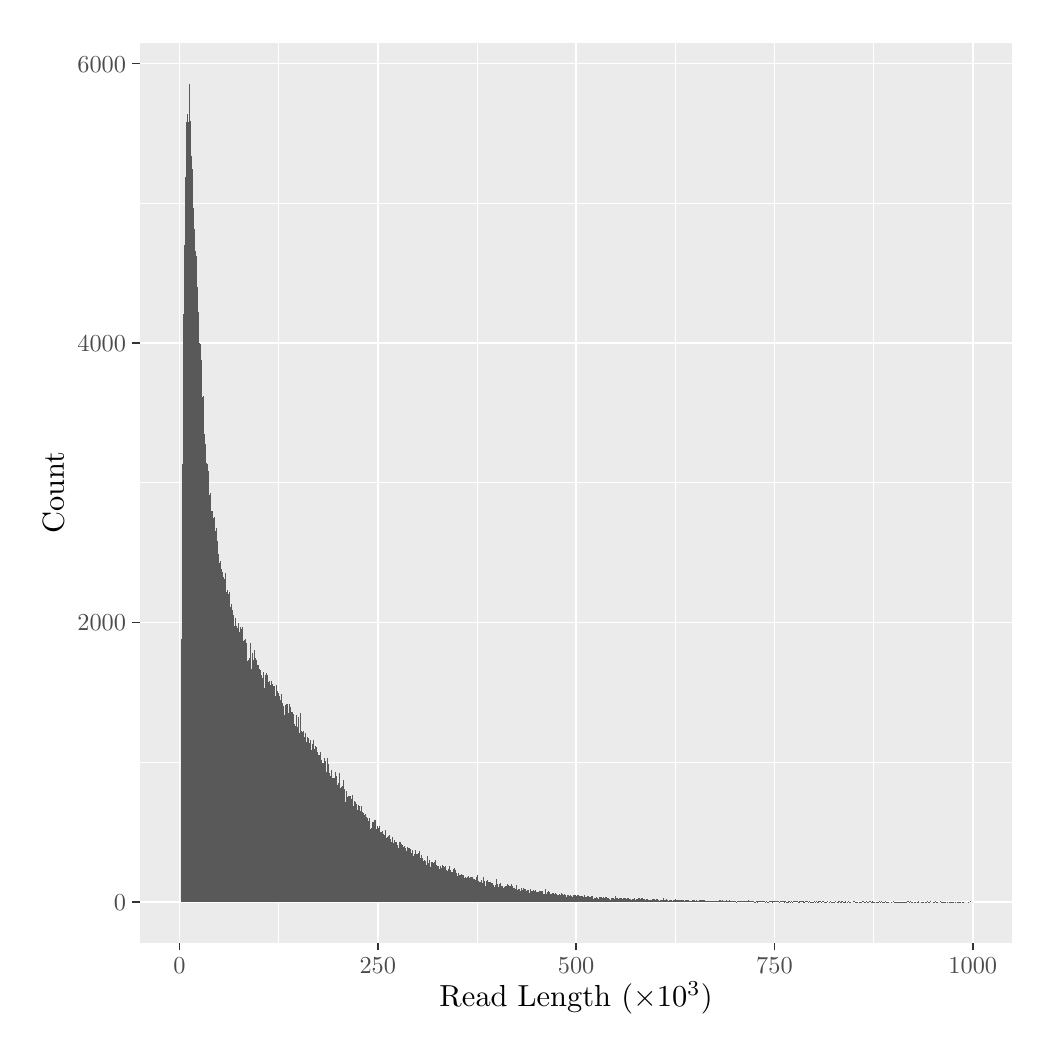
\begin{tikzpicture}[x=1pt,y=1pt]
\definecolor{fillColor}{RGB}{255,255,255}
\path[use as bounding box,fill=fillColor,fill opacity=0.00] (0,0) rectangle (361.35,361.35);
\begin{scope}
\path[clip] (  0.00,  0.00) rectangle (361.35,361.35);
\definecolor{drawColor}{RGB}{255,255,255}
\definecolor{fillColor}{RGB}{255,255,255}

\path[draw=drawColor,line width= 0.6pt,line join=round,line cap=round,fill=fillColor] (  0.00,  0.00) rectangle (361.35,361.35);
\end{scope}
\begin{scope}
\path[clip] ( 40.51, 30.69) rectangle (355.85,355.85);
\definecolor{fillColor}{gray}{0.92}

\path[fill=fillColor] ( 40.51, 30.69) rectangle (355.85,355.85);
\definecolor{drawColor}{RGB}{255,255,255}

\path[draw=drawColor,line width= 0.3pt,line join=round] ( 40.51, 95.94) --
	(355.85, 95.94);

\path[draw=drawColor,line width= 0.3pt,line join=round] ( 40.51,196.90) --
	(355.85,196.90);

\path[draw=drawColor,line width= 0.3pt,line join=round] ( 40.51,297.86) --
	(355.85,297.86);

\path[draw=drawColor,line width= 0.3pt,line join=round] ( 90.68, 30.69) --
	( 90.68,355.85);

\path[draw=drawColor,line width= 0.3pt,line join=round] (162.35, 30.69) --
	(162.35,355.85);

\path[draw=drawColor,line width= 0.3pt,line join=round] (234.01, 30.69) --
	(234.01,355.85);

\path[draw=drawColor,line width= 0.3pt,line join=round] (305.68, 30.69) --
	(305.68,355.85);

\path[draw=drawColor,line width= 0.6pt,line join=round] ( 40.51, 45.47) --
	(355.85, 45.47);

\path[draw=drawColor,line width= 0.6pt,line join=round] ( 40.51,146.42) --
	(355.85,146.42);

\path[draw=drawColor,line width= 0.6pt,line join=round] ( 40.51,247.38) --
	(355.85,247.38);

\path[draw=drawColor,line width= 0.6pt,line join=round] ( 40.51,348.34) --
	(355.85,348.34);

\path[draw=drawColor,line width= 0.6pt,line join=round] ( 54.84, 30.69) --
	( 54.84,355.85);

\path[draw=drawColor,line width= 0.6pt,line join=round] (126.51, 30.69) --
	(126.51,355.85);

\path[draw=drawColor,line width= 0.6pt,line join=round] (198.18, 30.69) --
	(198.18,355.85);

\path[draw=drawColor,line width= 0.6pt,line join=round] (269.85, 30.69) --
	(269.85,355.85);

\path[draw=drawColor,line width= 0.6pt,line join=round] (341.52, 30.69) --
	(341.52,355.85);
\definecolor{fillColor}{gray}{0.35}

\path[fill=fillColor] ( 54.99, 45.47) rectangle ( 55.27, 45.47);

\path[fill=fillColor] ( 55.27, 45.47) rectangle ( 55.56, 54.25);

\path[fill=fillColor] ( 55.56, 45.47) rectangle ( 55.85,140.62);

\path[fill=fillColor] ( 55.85, 45.47) rectangle ( 56.13,203.52);

\path[fill=fillColor] ( 56.13, 45.47) rectangle ( 56.42,257.73);

\path[fill=fillColor] ( 56.42, 45.47) rectangle ( 56.71,282.87);

\path[fill=fillColor] ( 56.71, 45.47) rectangle ( 56.99,307.25);

\path[fill=fillColor] ( 56.99, 45.47) rectangle ( 57.28,306.34);

\path[fill=fillColor] ( 57.28, 45.47) rectangle ( 57.57,327.24);

\path[fill=fillColor] ( 57.57, 45.47) rectangle ( 57.85,330.22);

\path[fill=fillColor] ( 57.85, 45.47) rectangle ( 58.14,327.44);

\path[fill=fillColor] ( 58.14, 45.47) rectangle ( 58.43,341.07);

\path[fill=fillColor] ( 58.43, 45.47) rectangle ( 58.71,334.61);

\path[fill=fillColor] ( 58.71, 45.47) rectangle ( 59.00,327.54);

\path[fill=fillColor] ( 59.00, 45.47) rectangle ( 59.29,314.82);

\path[fill=fillColor] ( 59.29, 45.47) rectangle ( 59.57,310.13);

\path[fill=fillColor] ( 59.57, 45.47) rectangle ( 59.86,292.26);

\path[fill=fillColor] ( 59.86, 45.47) rectangle ( 60.15,296.09);

\path[fill=fillColor] ( 60.15, 45.47) rectangle ( 60.43,288.77);

\path[fill=fillColor] ( 60.43, 45.47) rectangle ( 60.72,280.55);

\path[fill=fillColor] ( 60.72, 45.47) rectangle ( 61.01,278.68);

\path[fill=fillColor] ( 61.01, 45.47) rectangle ( 61.29,266.46);

\path[fill=fillColor] ( 61.29, 45.47) rectangle ( 61.58,267.47);

\path[fill=fillColor] ( 61.58, 45.47) rectangle ( 61.87,258.49);

\path[fill=fillColor] ( 61.87, 45.47) rectangle ( 62.15,247.33);

\path[fill=fillColor] ( 62.15, 45.47) rectangle ( 62.44,247.13);

\path[fill=fillColor] ( 62.44, 45.47) rectangle ( 62.73,244.60);

\path[fill=fillColor] ( 62.73, 45.47) rectangle ( 63.01,241.37);

\path[fill=fillColor] ( 63.01, 45.47) rectangle ( 63.30,227.85);

\path[fill=fillColor] ( 63.30, 45.47) rectangle ( 63.59,228.25);

\path[fill=fillColor] ( 63.59, 45.47) rectangle ( 63.87,214.17);

\path[fill=fillColor] ( 63.87, 45.47) rectangle ( 64.16,214.67);

\path[fill=fillColor] ( 64.16, 45.47) rectangle ( 64.45,210.94);

\path[fill=fillColor] ( 64.45, 45.47) rectangle ( 64.73,204.17);

\path[fill=fillColor] ( 64.73, 45.47) rectangle ( 65.02,203.72);

\path[fill=fillColor] ( 65.02, 45.47) rectangle ( 65.31,201.09);

\path[fill=fillColor] ( 65.31, 45.47) rectangle ( 65.59,199.38);

\path[fill=fillColor] ( 65.59, 45.47) rectangle ( 65.88,192.36);

\path[fill=fillColor] ( 65.88, 45.47) rectangle ( 66.17,193.27);

\path[fill=fillColor] ( 66.17, 45.47) rectangle ( 66.45,186.60);

\path[fill=fillColor] ( 66.45, 45.47) rectangle ( 66.74,182.82);

\path[fill=fillColor] ( 66.74, 45.47) rectangle ( 67.03,186.55);

\path[fill=fillColor] ( 67.03, 45.47) rectangle ( 67.31,184.18);

\path[fill=fillColor] ( 67.31, 45.47) rectangle ( 67.60,184.54);

\path[fill=fillColor] ( 67.60, 45.47) rectangle ( 67.89,179.39);

\path[fill=fillColor] ( 67.89, 45.47) rectangle ( 68.17,180.60);

\path[fill=fillColor] ( 68.17, 45.47) rectangle ( 68.46,175.25);

\path[fill=fillColor] ( 68.46, 45.47) rectangle ( 68.75,175.70);

\path[fill=fillColor] ( 68.75, 45.47) rectangle ( 69.03,171.16);

\path[fill=fillColor] ( 69.03, 45.47) rectangle ( 69.32,167.93);

\path[fill=fillColor] ( 69.32, 45.47) rectangle ( 69.61,168.58);

\path[fill=fillColor] ( 69.61, 45.47) rectangle ( 69.89,167.07);

\path[fill=fillColor] ( 69.89, 45.47) rectangle ( 70.18,165.66);

\path[fill=fillColor] ( 70.18, 45.47) rectangle ( 70.47,164.75);

\path[fill=fillColor] ( 70.47, 45.47) rectangle ( 70.75,162.78);

\path[fill=fillColor] ( 70.75, 45.47) rectangle ( 71.04,161.87);

\path[fill=fillColor] ( 71.04, 45.47) rectangle ( 71.33,162.02);

\path[fill=fillColor] ( 71.33, 45.47) rectangle ( 71.61,164.14);

\path[fill=fillColor] ( 71.61, 45.47) rectangle ( 71.90,157.28);

\path[fill=fillColor] ( 71.90, 45.47) rectangle ( 72.19,157.38);

\path[fill=fillColor] ( 72.19, 45.47) rectangle ( 72.47,158.13);

\path[fill=fillColor] ( 72.47, 45.47) rectangle ( 72.76,156.62);

\path[fill=fillColor] ( 72.76, 45.47) rectangle ( 73.05,157.38);

\path[fill=fillColor] ( 73.05, 45.47) rectangle ( 73.33,152.03);

\path[fill=fillColor] ( 73.33, 45.47) rectangle ( 73.62,150.41);

\path[fill=fillColor] ( 73.62, 45.47) rectangle ( 73.91,153.14);

\path[fill=fillColor] ( 73.91, 45.47) rectangle ( 74.19,150.87);

\path[fill=fillColor] ( 74.19, 45.47) rectangle ( 74.48,148.95);

\path[fill=fillColor] ( 74.48, 45.47) rectangle ( 74.77,145.31);

\path[fill=fillColor] ( 74.77, 45.47) rectangle ( 75.05,144.30);

\path[fill=fillColor] ( 75.05, 45.47) rectangle ( 75.34,148.04);

\path[fill=fillColor] ( 75.34, 45.47) rectangle ( 75.63,145.21);

\path[fill=fillColor] ( 75.63, 45.47) rectangle ( 75.91,144.56);

\path[fill=fillColor] ( 75.91, 45.47) rectangle ( 76.20,146.12);

\path[fill=fillColor] ( 76.20, 45.47) rectangle ( 76.49,142.18);

\path[fill=fillColor] ( 76.49, 45.47) rectangle ( 76.77,142.94);

\path[fill=fillColor] ( 76.77, 45.47) rectangle ( 77.06,144.86);

\path[fill=fillColor] ( 77.06, 45.47) rectangle ( 77.35,144.15);

\path[fill=fillColor] ( 77.35, 45.47) rectangle ( 77.63,144.76);

\path[fill=fillColor] ( 77.63, 45.47) rectangle ( 77.92,139.76);

\path[fill=fillColor] ( 77.92, 45.47) rectangle ( 78.21,138.95);

\path[fill=fillColor] ( 78.21, 45.47) rectangle ( 78.49,140.21);

\path[fill=fillColor] ( 78.49, 45.47) rectangle ( 78.78,140.52);

\path[fill=fillColor] ( 78.78, 45.47) rectangle ( 79.07,139.05);

\path[fill=fillColor] ( 79.07, 45.47) rectangle ( 79.35,131.48);

\path[fill=fillColor] ( 79.35, 45.47) rectangle ( 79.64,132.44);

\path[fill=fillColor] ( 79.64, 45.47) rectangle ( 79.93,132.74);

\path[fill=fillColor] ( 79.93, 45.47) rectangle ( 80.21,133.40);

\path[fill=fillColor] ( 80.21, 45.47) rectangle ( 80.50,135.67);

\path[fill=fillColor] ( 80.50, 45.47) rectangle ( 80.79,139.05);

\path[fill=fillColor] ( 80.79, 45.47) rectangle ( 81.07,129.77);

\path[fill=fillColor] ( 81.07, 45.47) rectangle ( 81.36,135.42);

\path[fill=fillColor] ( 81.36, 45.47) rectangle ( 81.65,132.90);

\path[fill=fillColor] ( 81.65, 45.47) rectangle ( 81.93,131.68);

\path[fill=fillColor] ( 81.93, 45.47) rectangle ( 82.22,136.38);

\path[fill=fillColor] ( 82.22, 45.47) rectangle ( 82.51,133.60);

\path[fill=fillColor] ( 82.51, 45.47) rectangle ( 82.79,132.90);

\path[fill=fillColor] ( 82.79, 45.47) rectangle ( 83.08,130.93);

\path[fill=fillColor] ( 83.08, 45.47) rectangle ( 83.37,131.08);

\path[fill=fillColor] ( 83.37, 45.47) rectangle ( 83.65,127.34);

\path[fill=fillColor] ( 83.65, 45.47) rectangle ( 83.94,129.77);

\path[fill=fillColor] ( 83.94, 45.47) rectangle ( 84.23,129.26);

\path[fill=fillColor] ( 84.23, 45.47) rectangle ( 84.51,127.54);

\path[fill=fillColor] ( 84.51, 45.47) rectangle ( 84.80,126.48);

\path[fill=fillColor] ( 84.80, 45.47) rectangle ( 85.09,123.51);

\path[fill=fillColor] ( 85.09, 45.47) rectangle ( 85.37,128.40);

\path[fill=fillColor] ( 85.37, 45.47) rectangle ( 85.66,122.80);

\path[fill=fillColor] ( 85.66, 45.47) rectangle ( 85.95,127.54);

\path[fill=fillColor] ( 85.95, 45.47) rectangle ( 86.23,125.27);

\path[fill=fillColor] ( 86.23, 45.47) rectangle ( 86.52,128.05);

\path[fill=fillColor] ( 86.52, 45.47) rectangle ( 86.81,127.49);

\path[fill=fillColor] ( 86.81, 45.47) rectangle ( 87.09,125.07);

\path[fill=fillColor] ( 87.09, 45.47) rectangle ( 87.38,123.51);

\path[fill=fillColor] ( 87.38, 45.47) rectangle ( 87.67,125.37);

\path[fill=fillColor] ( 87.67, 45.47) rectangle ( 87.95,123.71);

\path[fill=fillColor] ( 87.95, 45.47) rectangle ( 88.24,125.12);

\path[fill=fillColor] ( 88.24, 45.47) rectangle ( 88.53,124.11);

\path[fill=fillColor] ( 88.53, 45.47) rectangle ( 88.81,123.56);

\path[fill=fillColor] ( 88.81, 45.47) rectangle ( 89.10,122.55);

\path[fill=fillColor] ( 89.10, 45.47) rectangle ( 89.39,123.46);

\path[fill=fillColor] ( 89.39, 45.47) rectangle ( 89.67,119.87);

\path[fill=fillColor] ( 89.67, 45.47) rectangle ( 89.96,123.96);

\path[fill=fillColor] ( 89.96, 45.47) rectangle ( 90.25,121.74);

\path[fill=fillColor] ( 90.25, 45.47) rectangle ( 90.53,118.71);

\path[fill=fillColor] ( 90.53, 45.47) rectangle ( 90.82,121.03);

\path[fill=fillColor] ( 90.82, 45.47) rectangle ( 91.11,119.92);

\path[fill=fillColor] ( 91.11, 45.47) rectangle ( 91.39,118.56);

\path[fill=fillColor] ( 91.39, 45.47) rectangle ( 91.68,117.55);

\path[fill=fillColor] ( 91.68, 45.47) rectangle ( 91.97,120.58);

\path[fill=fillColor] ( 91.97, 45.47) rectangle ( 92.25,117.15);

\path[fill=fillColor] ( 92.25, 45.47) rectangle ( 92.54,116.14);

\path[fill=fillColor] ( 92.54, 45.47) rectangle ( 92.83,112.91);

\path[fill=fillColor] ( 92.83, 45.47) rectangle ( 93.11,114.37);

\path[fill=fillColor] ( 93.11, 45.47) rectangle ( 93.40,116.69);

\path[fill=fillColor] ( 93.40, 45.47) rectangle ( 93.69,116.79);

\path[fill=fillColor] ( 93.69, 45.47) rectangle ( 93.97,117.10);

\path[fill=fillColor] ( 93.97, 45.47) rectangle ( 94.26,113.76);

\path[fill=fillColor] ( 94.26, 45.47) rectangle ( 94.55,114.62);

\path[fill=fillColor] ( 94.55, 45.47) rectangle ( 94.83,116.94);

\path[fill=fillColor] ( 94.83, 45.47) rectangle ( 95.12,115.83);

\path[fill=fillColor] ( 95.12, 45.47) rectangle ( 95.41,113.92);

\path[fill=fillColor] ( 95.41, 45.47) rectangle ( 95.69,113.92);

\path[fill=fillColor] ( 95.69, 45.47) rectangle ( 95.98,108.72);

\path[fill=fillColor] ( 95.98, 45.47) rectangle ( 96.27,113.46);

\path[fill=fillColor] ( 96.27, 45.47) rectangle ( 96.55,109.73);

\path[fill=fillColor] ( 96.55, 45.47) rectangle ( 96.84,108.87);

\path[fill=fillColor] ( 96.84, 45.47) rectangle ( 97.13,112.86);

\path[fill=fillColor] ( 97.13, 45.47) rectangle ( 97.41,111.80);

\path[fill=fillColor] ( 97.41, 45.47) rectangle ( 97.70,108.72);

\path[fill=fillColor] ( 97.70, 45.47) rectangle ( 97.99,112.25);

\path[fill=fillColor] ( 97.99, 45.47) rectangle ( 98.27,106.65);

\path[fill=fillColor] ( 98.27, 45.47) rectangle ( 98.56,113.76);

\path[fill=fillColor] ( 98.56, 45.47) rectangle ( 98.85,106.34);

\path[fill=fillColor] ( 98.85, 45.47) rectangle ( 99.13,107.35);

\path[fill=fillColor] ( 99.13, 45.47) rectangle ( 99.42,107.00);

\path[fill=fillColor] ( 99.42, 45.47) rectangle ( 99.71,107.15);

\path[fill=fillColor] ( 99.71, 45.47) rectangle ( 99.99,105.13);

\path[fill=fillColor] ( 99.99, 45.47) rectangle (100.28,105.08);

\path[fill=fillColor] (100.28, 45.47) rectangle (100.57,106.34);

\path[fill=fillColor] (100.57, 45.47) rectangle (100.85,103.26);

\path[fill=fillColor] (100.85, 45.47) rectangle (101.14,104.93);

\path[fill=fillColor] (101.14, 45.47) rectangle (101.43,104.68);

\path[fill=fillColor] (101.43, 45.47) rectangle (101.71,102.25);

\path[fill=fillColor] (101.71, 45.47) rectangle (102.00,102.96);

\path[fill=fillColor] (102.00, 45.47) rectangle (102.29,103.87);

\path[fill=fillColor] (102.29, 45.47) rectangle (102.57,100.39);

\path[fill=fillColor] (102.57, 45.47) rectangle (102.86,102.61);

\path[fill=fillColor] (102.86, 45.47) rectangle (103.15,102.61);

\path[fill=fillColor] (103.15, 45.47) rectangle (103.43,104.12);

\path[fill=fillColor] (103.43, 45.47) rectangle (103.72,100.74);

\path[fill=fillColor] (103.72, 45.47) rectangle (104.01,101.85);

\path[fill=fillColor] (104.01, 45.47) rectangle (104.29,100.29);

\path[fill=fillColor] (104.29, 45.47) rectangle (104.58,101.35);

\path[fill=fillColor] (104.58, 45.47) rectangle (104.87, 99.53);

\path[fill=fillColor] (104.87, 45.47) rectangle (105.15, 98.52);

\path[fill=fillColor] (105.15, 45.47) rectangle (105.44, 98.47);

\path[fill=fillColor] (105.44, 45.47) rectangle (105.73, 97.00);

\path[fill=fillColor] (105.73, 45.47) rectangle (106.01, 99.73);

\path[fill=fillColor] (106.01, 45.47) rectangle (106.30, 96.80);

\path[fill=fillColor] (106.30, 45.47) rectangle (106.59, 95.64);

\path[fill=fillColor] (106.59, 45.47) rectangle (106.87, 95.79);

\path[fill=fillColor] (106.87, 45.47) rectangle (107.16, 93.93);

\path[fill=fillColor] (107.16, 45.47) rectangle (107.45, 97.61);

\path[fill=fillColor] (107.45, 45.47) rectangle (107.73, 96.45);

\path[fill=fillColor] (107.73, 45.47) rectangle (108.02, 92.41);

\path[fill=fillColor] (108.02, 45.47) rectangle (108.31, 97.46);

\path[fill=fillColor] (108.31, 45.47) rectangle (108.59, 92.82);

\path[fill=fillColor] (108.59, 45.47) rectangle (108.88, 95.19);

\path[fill=fillColor] (108.88, 45.47) rectangle (109.17, 91.96);

\path[fill=fillColor] (109.17, 45.47) rectangle (109.45, 90.80);

\path[fill=fillColor] (109.45, 45.47) rectangle (109.74, 91.86);

\path[fill=fillColor] (109.74, 45.47) rectangle (110.03, 93.02);

\path[fill=fillColor] (110.03, 45.47) rectangle (110.31, 90.24);

\path[fill=fillColor] (110.31, 45.47) rectangle (110.60, 90.14);

\path[fill=fillColor] (110.60, 45.47) rectangle (110.89, 90.04);

\path[fill=fillColor] (110.89, 45.47) rectangle (111.17, 92.31);

\path[fill=fillColor] (111.17, 45.47) rectangle (111.46, 89.08);

\path[fill=fillColor] (111.46, 45.47) rectangle (111.75, 91.10);

\path[fill=fillColor] (111.75, 45.47) rectangle (112.03, 87.51);

\path[fill=fillColor] (112.03, 45.47) rectangle (112.32, 88.47);

\path[fill=fillColor] (112.32, 45.47) rectangle (112.61, 91.96);

\path[fill=fillColor] (112.61, 45.47) rectangle (112.89, 86.20);

\path[fill=fillColor] (112.89, 45.47) rectangle (113.18, 86.71);

\path[fill=fillColor] (113.18, 45.47) rectangle (113.47, 86.81);

\path[fill=fillColor] (113.47, 45.47) rectangle (113.75, 87.16);

\path[fill=fillColor] (113.75, 45.47) rectangle (114.04, 84.64);

\path[fill=fillColor] (114.04, 45.47) rectangle (114.33, 89.38);

\path[fill=fillColor] (114.33, 45.47) rectangle (114.61, 86.30);

\path[fill=fillColor] (114.61, 45.47) rectangle (114.90, 81.66);

\path[fill=fillColor] (114.90, 45.47) rectangle (115.19, 85.45);

\path[fill=fillColor] (115.19, 45.47) rectangle (115.48, 84.54);

\path[fill=fillColor] (115.48, 45.47) rectangle (115.76, 83.53);

\path[fill=fillColor] (115.76, 45.47) rectangle (116.05, 83.63);

\path[fill=fillColor] (116.05, 45.47) rectangle (116.34, 83.78);

\path[fill=fillColor] (116.34, 45.47) rectangle (116.62, 83.17);

\path[fill=fillColor] (116.62, 45.47) rectangle (116.91, 83.73);

\path[fill=fillColor] (116.91, 45.47) rectangle (117.20, 82.57);

\path[fill=fillColor] (117.20, 45.47) rectangle (117.48, 84.03);

\path[fill=fillColor] (117.48, 45.47) rectangle (117.77, 80.04);

\path[fill=fillColor] (117.77, 45.47) rectangle (118.06, 79.54);

\path[fill=fillColor] (118.06, 45.47) rectangle (118.34, 81.81);

\path[fill=fillColor] (118.34, 45.47) rectangle (118.63, 81.56);

\path[fill=fillColor] (118.63, 45.47) rectangle (118.92, 80.70);

\path[fill=fillColor] (118.92, 45.47) rectangle (119.20, 78.73);

\path[fill=fillColor] (119.20, 45.47) rectangle (119.49, 79.08);

\path[fill=fillColor] (119.49, 45.47) rectangle (119.78, 80.30);

\path[fill=fillColor] (119.78, 45.47) rectangle (120.06, 80.09);

\path[fill=fillColor] (120.06, 45.47) rectangle (120.35, 78.28);

\path[fill=fillColor] (120.35, 45.47) rectangle (120.64, 80.20);

\path[fill=fillColor] (120.64, 45.47) rectangle (120.92, 77.77);

\path[fill=fillColor] (120.92, 45.47) rectangle (121.21, 75.85);

\path[fill=fillColor] (121.21, 45.47) rectangle (121.50, 77.67);

\path[fill=fillColor] (121.50, 45.47) rectangle (121.78, 76.96);

\path[fill=fillColor] (121.78, 45.47) rectangle (122.07, 77.12);

\path[fill=fillColor] (122.07, 45.47) rectangle (122.36, 77.07);

\path[fill=fillColor] (122.36, 45.47) rectangle (122.64, 76.26);

\path[fill=fillColor] (122.64, 45.47) rectangle (122.93, 75.70);

\path[fill=fillColor] (122.93, 45.47) rectangle (123.22, 74.69);

\path[fill=fillColor] (123.22, 45.47) rectangle (123.50, 75.60);

\path[fill=fillColor] (123.50, 45.47) rectangle (123.79, 75.25);

\path[fill=fillColor] (123.79, 45.47) rectangle (124.08, 71.66);

\path[fill=fillColor] (124.08, 45.47) rectangle (124.36, 71.97);

\path[fill=fillColor] (124.36, 45.47) rectangle (124.65, 74.44);

\path[fill=fillColor] (124.65, 45.47) rectangle (124.94, 74.29);

\path[fill=fillColor] (124.94, 45.47) rectangle (125.22, 73.28);

\path[fill=fillColor] (125.22, 45.47) rectangle (125.51, 74.90);

\path[fill=fillColor] (125.51, 45.47) rectangle (125.80, 75.00);

\path[fill=fillColor] (125.80, 45.47) rectangle (126.08, 71.66);

\path[fill=fillColor] (126.08, 45.47) rectangle (126.37, 72.88);

\path[fill=fillColor] (126.37, 45.47) rectangle (126.66, 71.77);

\path[fill=fillColor] (126.66, 45.47) rectangle (126.94, 71.97);

\path[fill=fillColor] (126.94, 45.47) rectangle (127.23, 72.78);

\path[fill=fillColor] (127.23, 45.47) rectangle (127.52, 70.81);

\path[fill=fillColor] (127.52, 45.47) rectangle (127.80, 70.45);

\path[fill=fillColor] (127.80, 45.47) rectangle (128.09, 70.86);

\path[fill=fillColor] (128.09, 45.47) rectangle (128.38, 70.96);

\path[fill=fillColor] (128.38, 45.47) rectangle (128.66, 70.10);

\path[fill=fillColor] (128.66, 45.47) rectangle (128.95, 69.80);

\path[fill=fillColor] (128.95, 45.47) rectangle (129.24, 71.46);

\path[fill=fillColor] (129.24, 45.47) rectangle (129.52, 69.29);

\path[fill=fillColor] (129.52, 45.47) rectangle (129.81, 68.64);

\path[fill=fillColor] (129.81, 45.47) rectangle (130.10, 68.84);

\path[fill=fillColor] (130.10, 45.47) rectangle (130.38, 69.09);

\path[fill=fillColor] (130.38, 45.47) rectangle (130.67, 66.52);

\path[fill=fillColor] (130.67, 45.47) rectangle (130.96, 69.75);

\path[fill=fillColor] (130.96, 45.47) rectangle (131.24, 68.18);

\path[fill=fillColor] (131.24, 45.47) rectangle (131.53, 66.92);

\path[fill=fillColor] (131.53, 45.47) rectangle (131.82, 68.84);

\path[fill=fillColor] (131.82, 45.47) rectangle (132.10, 68.74);

\path[fill=fillColor] (132.10, 45.47) rectangle (132.39, 66.87);

\path[fill=fillColor] (132.39, 45.47) rectangle (132.68, 67.68);

\path[fill=fillColor] (132.68, 45.47) rectangle (132.96, 67.27);

\path[fill=fillColor] (132.96, 45.47) rectangle (133.25, 67.07);

\path[fill=fillColor] (133.25, 45.47) rectangle (133.54, 66.06);

\path[fill=fillColor] (133.54, 45.47) rectangle (133.82, 65.86);

\path[fill=fillColor] (133.82, 45.47) rectangle (134.11, 64.85);

\path[fill=fillColor] (134.11, 45.47) rectangle (134.40, 67.22);

\path[fill=fillColor] (134.40, 45.47) rectangle (134.68, 65.41);

\path[fill=fillColor] (134.68, 45.47) rectangle (134.97, 67.27);

\path[fill=fillColor] (134.97, 45.47) rectangle (135.26, 66.47);

\path[fill=fillColor] (135.26, 45.47) rectangle (135.54, 65.96);

\path[fill=fillColor] (135.54, 45.47) rectangle (135.83, 65.41);

\path[fill=fillColor] (135.83, 45.47) rectangle (136.12, 64.29);

\path[fill=fillColor] (136.12, 45.47) rectangle (136.40, 65.81);

\path[fill=fillColor] (136.40, 45.47) rectangle (136.69, 65.00);

\path[fill=fillColor] (136.69, 45.47) rectangle (136.98, 63.74);

\path[fill=fillColor] (136.98, 45.47) rectangle (137.26, 65.35);

\path[fill=fillColor] (137.26, 45.47) rectangle (137.55, 64.80);

\path[fill=fillColor] (137.55, 45.47) rectangle (137.84, 63.49);

\path[fill=fillColor] (137.84, 45.47) rectangle (138.12, 64.75);

\path[fill=fillColor] (138.12, 45.47) rectangle (138.41, 64.40);

\path[fill=fillColor] (138.41, 45.47) rectangle (138.70, 63.23);

\path[fill=fillColor] (138.70, 45.47) rectangle (138.98, 64.09);

\path[fill=fillColor] (138.98, 45.47) rectangle (139.27, 63.84);

\path[fill=fillColor] (139.27, 45.47) rectangle (139.56, 62.02);

\path[fill=fillColor] (139.56, 45.47) rectangle (139.84, 62.68);

\path[fill=fillColor] (139.84, 45.47) rectangle (140.13, 64.19);

\path[fill=fillColor] (140.13, 45.47) rectangle (140.42, 60.81);

\path[fill=fillColor] (140.42, 45.47) rectangle (140.70, 62.58);

\path[fill=fillColor] (140.70, 45.47) rectangle (140.99, 62.73);

\path[fill=fillColor] (140.99, 45.47) rectangle (141.28, 63.13);

\path[fill=fillColor] (141.28, 45.47) rectangle (141.56, 63.94);

\path[fill=fillColor] (141.56, 45.47) rectangle (141.85, 63.59);

\path[fill=fillColor] (141.85, 45.47) rectangle (142.14, 61.22);

\path[fill=fillColor] (142.14, 45.47) rectangle (142.42, 62.33);

\path[fill=fillColor] (142.42, 45.47) rectangle (142.71, 61.22);

\path[fill=fillColor] (142.71, 45.47) rectangle (143.00, 60.31);

\path[fill=fillColor] (143.00, 45.47) rectangle (143.28, 60.26);

\path[fill=fillColor] (143.28, 45.47) rectangle (143.57, 60.46);

\path[fill=fillColor] (143.57, 45.47) rectangle (143.86, 60.31);

\path[fill=fillColor] (143.86, 45.47) rectangle (144.14, 58.79);

\path[fill=fillColor] (144.14, 45.47) rectangle (144.43, 60.91);

\path[fill=fillColor] (144.43, 45.47) rectangle (144.72, 61.87);

\path[fill=fillColor] (144.72, 45.47) rectangle (145.00, 59.35);

\path[fill=fillColor] (145.00, 45.47) rectangle (145.29, 60.71);

\path[fill=fillColor] (145.29, 45.47) rectangle (145.58, 57.88);

\path[fill=fillColor] (145.58, 45.47) rectangle (145.86, 60.00);

\path[fill=fillColor] (145.86, 45.47) rectangle (146.15, 58.59);

\path[fill=fillColor] (146.15, 45.47) rectangle (146.44, 59.85);

\path[fill=fillColor] (146.44, 45.47) rectangle (146.72, 59.35);

\path[fill=fillColor] (146.72, 45.47) rectangle (147.01, 59.75);

\path[fill=fillColor] (147.01, 45.47) rectangle (147.30, 60.56);

\path[fill=fillColor] (147.30, 45.47) rectangle (147.58, 57.48);

\path[fill=fillColor] (147.58, 45.47) rectangle (147.87, 58.74);

\path[fill=fillColor] (147.87, 45.47) rectangle (148.16, 58.39);

\path[fill=fillColor] (148.16, 45.47) rectangle (148.44, 57.03);

\path[fill=fillColor] (148.44, 45.47) rectangle (148.73, 58.59);

\path[fill=fillColor] (148.73, 45.47) rectangle (149.02, 57.28);

\path[fill=fillColor] (149.02, 45.47) rectangle (149.30, 58.49);

\path[fill=fillColor] (149.30, 45.47) rectangle (149.59, 57.63);

\path[fill=fillColor] (149.59, 45.47) rectangle (149.88, 58.79);

\path[fill=fillColor] (149.88, 45.47) rectangle (150.16, 58.69);

\path[fill=fillColor] (150.16, 45.47) rectangle (150.45, 58.59);

\path[fill=fillColor] (150.45, 45.47) rectangle (150.74, 57.93);

\path[fill=fillColor] (150.74, 45.47) rectangle (151.02, 58.29);

\path[fill=fillColor] (151.02, 45.47) rectangle (151.31, 57.08);

\path[fill=fillColor] (151.31, 45.47) rectangle (151.60, 56.12);

\path[fill=fillColor] (151.60, 45.47) rectangle (151.88, 56.47);

\path[fill=fillColor] (151.88, 45.47) rectangle (152.17, 57.38);

\path[fill=fillColor] (152.17, 45.47) rectangle (152.46, 58.24);

\path[fill=fillColor] (152.46, 45.47) rectangle (152.74, 56.67);

\path[fill=fillColor] (152.74, 45.47) rectangle (153.03, 56.92);

\path[fill=fillColor] (153.03, 45.47) rectangle (153.32, 56.22);

\path[fill=fillColor] (153.32, 45.47) rectangle (153.60, 56.17);

\path[fill=fillColor] (153.60, 45.47) rectangle (153.89, 57.48);

\path[fill=fillColor] (153.89, 45.47) rectangle (154.18, 57.63);

\path[fill=fillColor] (154.18, 45.47) rectangle (154.46, 54.50);

\path[fill=fillColor] (154.46, 45.47) rectangle (154.75, 57.13);

\path[fill=fillColor] (154.75, 45.47) rectangle (155.04, 56.02);

\path[fill=fillColor] (155.04, 45.47) rectangle (155.32, 54.65);

\path[fill=fillColor] (155.32, 45.47) rectangle (155.61, 56.07);

\path[fill=fillColor] (155.61, 45.47) rectangle (155.90, 55.16);

\path[fill=fillColor] (155.90, 45.47) rectangle (156.18, 55.16);

\path[fill=fillColor] (156.18, 45.47) rectangle (156.47, 55.06);

\path[fill=fillColor] (156.47, 45.47) rectangle (156.76, 54.55);

\path[fill=fillColor] (156.76, 45.47) rectangle (157.04, 55.51);

\path[fill=fillColor] (157.04, 45.47) rectangle (157.33, 55.01);

\path[fill=fillColor] (157.33, 45.47) rectangle (157.62, 55.06);

\path[fill=fillColor] (157.62, 45.47) rectangle (157.90, 54.05);

\path[fill=fillColor] (157.90, 45.47) rectangle (158.19, 54.35);

\path[fill=fillColor] (158.19, 45.47) rectangle (158.48, 54.10);

\path[fill=fillColor] (158.48, 45.47) rectangle (158.76, 54.15);

\path[fill=fillColor] (158.76, 45.47) rectangle (159.05, 54.30);

\path[fill=fillColor] (159.05, 45.47) rectangle (159.34, 54.70);

\path[fill=fillColor] (159.34, 45.47) rectangle (159.62, 53.69);

\path[fill=fillColor] (159.62, 45.47) rectangle (159.91, 54.10);

\path[fill=fillColor] (159.91, 45.47) rectangle (160.20, 54.30);

\path[fill=fillColor] (160.20, 45.47) rectangle (160.48, 54.30);

\path[fill=fillColor] (160.48, 45.47) rectangle (160.77, 54.35);

\path[fill=fillColor] (160.77, 45.47) rectangle (161.06, 53.54);

\path[fill=fillColor] (161.06, 45.47) rectangle (161.34, 53.69);

\path[fill=fillColor] (161.34, 45.47) rectangle (161.63, 53.90);

\path[fill=fillColor] (161.63, 45.47) rectangle (161.92, 53.24);

\path[fill=fillColor] (161.92, 45.47) rectangle (162.20, 54.55);

\path[fill=fillColor] (162.20, 45.47) rectangle (162.49, 53.59);

\path[fill=fillColor] (162.49, 45.47) rectangle (162.78, 55.01);

\path[fill=fillColor] (162.78, 45.47) rectangle (163.06, 53.04);

\path[fill=fillColor] (163.06, 45.47) rectangle (163.35, 52.48);

\path[fill=fillColor] (163.35, 45.47) rectangle (163.64, 52.68);

\path[fill=fillColor] (163.64, 45.47) rectangle (163.92, 53.54);

\path[fill=fillColor] (163.92, 45.47) rectangle (164.21, 53.24);

\path[fill=fillColor] (164.21, 45.47) rectangle (164.50, 52.43);

\path[fill=fillColor] (164.50, 45.47) rectangle (164.78, 54.45);

\path[fill=fillColor] (164.78, 45.47) rectangle (165.07, 52.58);

\path[fill=fillColor] (165.07, 45.47) rectangle (165.36, 52.99);

\path[fill=fillColor] (165.36, 45.47) rectangle (165.64, 51.32);

\path[fill=fillColor] (165.64, 45.47) rectangle (165.93, 53.09);

\path[fill=fillColor] (165.93, 45.47) rectangle (166.22, 53.19);

\path[fill=fillColor] (166.22, 45.47) rectangle (166.50, 51.73);

\path[fill=fillColor] (166.50, 45.47) rectangle (166.79, 52.68);

\path[fill=fillColor] (166.79, 45.47) rectangle (167.08, 52.68);

\path[fill=fillColor] (167.08, 45.47) rectangle (167.36, 52.53);

\path[fill=fillColor] (167.36, 45.47) rectangle (167.65, 52.13);

\path[fill=fillColor] (167.65, 45.47) rectangle (167.94, 52.28);

\path[fill=fillColor] (167.94, 45.47) rectangle (168.22, 51.88);

\path[fill=fillColor] (168.22, 45.47) rectangle (168.51, 51.47);

\path[fill=fillColor] (168.51, 45.47) rectangle (168.80, 50.97);

\path[fill=fillColor] (168.80, 45.47) rectangle (169.08, 51.52);

\path[fill=fillColor] (169.08, 45.47) rectangle (169.37, 51.02);

\path[fill=fillColor] (169.37, 45.47) rectangle (169.66, 53.80);

\path[fill=fillColor] (169.66, 45.47) rectangle (169.94, 51.78);

\path[fill=fillColor] (169.94, 45.47) rectangle (170.23, 50.97);

\path[fill=fillColor] (170.23, 45.47) rectangle (170.52, 51.83);

\path[fill=fillColor] (170.52, 45.47) rectangle (170.80, 52.28);

\path[fill=fillColor] (170.80, 45.47) rectangle (171.09, 51.62);

\path[fill=fillColor] (171.09, 45.47) rectangle (171.38, 51.12);

\path[fill=fillColor] (171.38, 45.47) rectangle (171.66, 51.02);

\path[fill=fillColor] (171.66, 45.47) rectangle (171.95, 50.51);

\path[fill=fillColor] (171.95, 45.47) rectangle (172.24, 50.87);

\path[fill=fillColor] (172.24, 45.47) rectangle (172.52, 50.36);

\path[fill=fillColor] (172.52, 45.47) rectangle (172.81, 51.27);

\path[fill=fillColor] (172.81, 45.47) rectangle (173.10, 51.27);

\path[fill=fillColor] (173.10, 45.47) rectangle (173.38, 50.51);

\path[fill=fillColor] (173.38, 45.47) rectangle (173.67, 52.03);

\path[fill=fillColor] (173.67, 45.47) rectangle (173.96, 51.52);

\path[fill=fillColor] (173.96, 45.47) rectangle (174.24, 51.12);

\path[fill=fillColor] (174.24, 45.47) rectangle (174.53, 51.02);

\path[fill=fillColor] (174.53, 45.47) rectangle (174.82, 51.78);

\path[fill=fillColor] (174.82, 45.47) rectangle (175.10, 51.02);

\path[fill=fillColor] (175.10, 45.47) rectangle (175.39, 51.22);

\path[fill=fillColor] (175.39, 45.47) rectangle (175.68, 50.61);

\path[fill=fillColor] (175.68, 45.47) rectangle (175.96, 50.31);

\path[fill=fillColor] (175.96, 45.47) rectangle (176.25, 50.26);

\path[fill=fillColor] (176.25, 45.47) rectangle (176.54, 49.40);

\path[fill=fillColor] (176.54, 45.47) rectangle (176.82, 51.47);

\path[fill=fillColor] (176.82, 45.47) rectangle (177.11, 49.76);

\path[fill=fillColor] (177.11, 45.47) rectangle (177.40, 50.16);

\path[fill=fillColor] (177.40, 45.47) rectangle (177.68, 49.86);

\path[fill=fillColor] (177.68, 45.47) rectangle (177.97, 50.06);

\path[fill=fillColor] (177.97, 45.47) rectangle (178.26, 49.45);

\path[fill=fillColor] (178.26, 45.47) rectangle (178.54, 50.61);

\path[fill=fillColor] (178.54, 45.47) rectangle (178.83, 49.71);

\path[fill=fillColor] (178.83, 45.47) rectangle (179.12, 50.56);

\path[fill=fillColor] (179.12, 45.47) rectangle (179.40, 49.76);

\path[fill=fillColor] (179.40, 45.47) rectangle (179.69, 50.11);

\path[fill=fillColor] (179.69, 45.47) rectangle (179.98, 50.01);

\path[fill=fillColor] (179.98, 45.47) rectangle (180.26, 49.45);

\path[fill=fillColor] (180.26, 45.47) rectangle (180.55, 49.61);

\path[fill=fillColor] (180.55, 45.47) rectangle (180.84, 48.70);

\path[fill=fillColor] (180.84, 45.47) rectangle (181.12, 49.76);

\path[fill=fillColor] (181.12, 45.47) rectangle (181.41, 48.80);

\path[fill=fillColor] (181.41, 45.47) rectangle (181.70, 49.96);

\path[fill=fillColor] (181.70, 45.47) rectangle (181.98, 49.25);

\path[fill=fillColor] (181.98, 45.47) rectangle (182.27, 49.15);

\path[fill=fillColor] (182.27, 45.47) rectangle (182.56, 49.40);

\path[fill=fillColor] (182.56, 45.47) rectangle (182.84, 49.61);

\path[fill=fillColor] (182.84, 45.47) rectangle (183.13, 49.25);

\path[fill=fillColor] (183.13, 45.47) rectangle (183.42, 49.30);

\path[fill=fillColor] (183.42, 45.47) rectangle (183.70, 49.66);

\path[fill=fillColor] (183.70, 45.47) rectangle (183.99, 49.15);

\path[fill=fillColor] (183.99, 45.47) rectangle (184.28, 49.15);

\path[fill=fillColor] (184.28, 45.47) rectangle (184.56, 49.10);

\path[fill=fillColor] (184.56, 45.47) rectangle (184.85, 49.05);

\path[fill=fillColor] (184.85, 45.47) rectangle (185.14, 49.55);

\path[fill=fillColor] (185.14, 45.47) rectangle (185.42, 49.25);

\path[fill=fillColor] (185.42, 45.47) rectangle (185.71, 49.45);

\path[fill=fillColor] (185.71, 45.47) rectangle (186.00, 48.65);

\path[fill=fillColor] (186.00, 45.47) rectangle (186.28, 49.25);

\path[fill=fillColor] (186.28, 45.47) rectangle (186.57, 48.39);

\path[fill=fillColor] (186.57, 45.47) rectangle (186.86, 48.29);

\path[fill=fillColor] (186.86, 45.47) rectangle (187.14, 49.96);

\path[fill=fillColor] (187.14, 45.47) rectangle (187.43, 48.29);

\path[fill=fillColor] (187.43, 45.47) rectangle (187.72, 48.29);

\path[fill=fillColor] (187.72, 45.47) rectangle (188.00, 49.00);

\path[fill=fillColor] (188.00, 45.47) rectangle (188.29, 49.50);

\path[fill=fillColor] (188.29, 45.47) rectangle (188.58, 49.05);

\path[fill=fillColor] (188.58, 45.47) rectangle (188.86, 47.99);

\path[fill=fillColor] (188.86, 45.47) rectangle (189.15, 48.29);

\path[fill=fillColor] (189.15, 45.47) rectangle (189.44, 48.29);

\path[fill=fillColor] (189.44, 45.47) rectangle (189.72, 48.75);

\path[fill=fillColor] (189.72, 45.47) rectangle (190.01, 48.55);

\path[fill=fillColor] (190.01, 45.47) rectangle (190.30, 48.09);

\path[fill=fillColor] (190.30, 45.47) rectangle (190.58, 48.44);

\path[fill=fillColor] (190.58, 45.47) rectangle (190.87, 48.55);

\path[fill=fillColor] (190.87, 45.47) rectangle (191.16, 48.14);

\path[fill=fillColor] (191.16, 45.47) rectangle (191.44, 48.04);

\path[fill=fillColor] (191.44, 45.47) rectangle (191.73, 47.79);

\path[fill=fillColor] (191.73, 45.47) rectangle (192.02, 48.04);

\path[fill=fillColor] (192.02, 45.47) rectangle (192.30, 48.19);

\path[fill=fillColor] (192.30, 45.47) rectangle (192.59, 47.94);

\path[fill=fillColor] (192.59, 45.47) rectangle (192.88, 48.39);

\path[fill=fillColor] (192.88, 45.47) rectangle (193.16, 48.55);

\path[fill=fillColor] (193.16, 45.47) rectangle (193.45, 48.24);

\path[fill=fillColor] (193.45, 45.47) rectangle (193.74, 47.94);

\path[fill=fillColor] (193.74, 45.47) rectangle (194.02, 48.34);

\path[fill=fillColor] (194.02, 45.47) rectangle (194.31, 47.94);

\path[fill=fillColor] (194.31, 45.47) rectangle (194.60, 47.79);

\path[fill=fillColor] (194.60, 45.47) rectangle (194.88, 47.28);

\path[fill=fillColor] (194.88, 45.47) rectangle (195.17, 48.04);

\path[fill=fillColor] (195.17, 45.47) rectangle (195.46, 47.94);

\path[fill=fillColor] (195.46, 45.47) rectangle (195.74, 47.59);

\path[fill=fillColor] (195.74, 45.47) rectangle (196.03, 47.74);

\path[fill=fillColor] (196.03, 45.47) rectangle (196.32, 47.94);

\path[fill=fillColor] (196.32, 45.47) rectangle (196.60, 47.59);

\path[fill=fillColor] (196.60, 45.47) rectangle (196.89, 47.23);

\path[fill=fillColor] (196.89, 45.47) rectangle (197.18, 47.99);

\path[fill=fillColor] (197.18, 45.47) rectangle (197.46, 47.64);

\path[fill=fillColor] (197.46, 45.47) rectangle (197.75, 47.94);

\path[fill=fillColor] (197.75, 45.47) rectangle (198.04, 47.89);

\path[fill=fillColor] (198.04, 45.47) rectangle (198.32, 47.54);

\path[fill=fillColor] (198.32, 45.47) rectangle (198.61, 47.94);

\path[fill=fillColor] (198.61, 45.47) rectangle (198.90, 47.79);

\path[fill=fillColor] (198.90, 45.47) rectangle (199.18, 47.79);

\path[fill=fillColor] (199.18, 45.47) rectangle (199.47, 47.49);

\path[fill=fillColor] (199.47, 45.47) rectangle (199.76, 47.43);

\path[fill=fillColor] (199.76, 45.47) rectangle (200.04, 47.33);

\path[fill=fillColor] (200.04, 45.47) rectangle (200.33, 47.49);

\path[fill=fillColor] (200.33, 45.47) rectangle (200.62, 47.69);

\path[fill=fillColor] (200.62, 45.47) rectangle (200.90, 47.18);

\path[fill=fillColor] (200.90, 45.47) rectangle (201.19, 47.84);

\path[fill=fillColor] (201.19, 45.47) rectangle (201.48, 47.18);

\path[fill=fillColor] (201.48, 45.47) rectangle (201.76, 47.23);

\path[fill=fillColor] (201.76, 45.47) rectangle (202.05, 47.23);

\path[fill=fillColor] (202.05, 45.47) rectangle (202.34, 47.43);

\path[fill=fillColor] (202.34, 45.47) rectangle (202.62, 47.28);

\path[fill=fillColor] (202.62, 45.47) rectangle (202.91, 47.43);

\path[fill=fillColor] (202.91, 45.47) rectangle (203.20, 47.38);

\path[fill=fillColor] (203.20, 45.47) rectangle (203.48, 47.13);

\path[fill=fillColor] (203.48, 45.47) rectangle (203.77, 47.59);

\path[fill=fillColor] (203.77, 45.47) rectangle (204.06, 47.49);

\path[fill=fillColor] (204.06, 45.47) rectangle (204.34, 47.64);

\path[fill=fillColor] (204.34, 45.47) rectangle (204.63, 46.48);

\path[fill=fillColor] (204.63, 45.47) rectangle (204.92, 46.98);

\path[fill=fillColor] (204.92, 45.47) rectangle (205.20, 46.68);

\path[fill=fillColor] (205.20, 45.47) rectangle (205.49, 47.28);

\path[fill=fillColor] (205.49, 45.47) rectangle (205.78, 47.23);

\path[fill=fillColor] (205.78, 45.47) rectangle (206.06, 46.73);

\path[fill=fillColor] (206.06, 45.47) rectangle (206.35, 46.53);

\path[fill=fillColor] (206.35, 45.47) rectangle (206.64, 47.38);

\path[fill=fillColor] (206.64, 45.47) rectangle (206.92, 47.38);

\path[fill=fillColor] (206.92, 45.47) rectangle (207.21, 47.13);

\path[fill=fillColor] (207.21, 45.47) rectangle (207.50, 47.23);

\path[fill=fillColor] (207.50, 45.47) rectangle (207.78, 46.68);

\path[fill=fillColor] (207.78, 45.47) rectangle (208.07, 46.63);

\path[fill=fillColor] (208.07, 45.47) rectangle (208.36, 47.28);

\path[fill=fillColor] (208.36, 45.47) rectangle (208.64, 46.98);

\path[fill=fillColor] (208.64, 45.47) rectangle (208.93, 47.13);

\path[fill=fillColor] (208.93, 45.47) rectangle (209.22, 47.08);

\path[fill=fillColor] (209.22, 45.47) rectangle (209.50, 46.68);

\path[fill=fillColor] (209.50, 45.47) rectangle (209.79, 46.68);

\path[fill=fillColor] (209.79, 45.47) rectangle (210.08, 46.83);

\path[fill=fillColor] (210.08, 45.47) rectangle (210.36, 46.32);

\path[fill=fillColor] (210.36, 45.47) rectangle (210.65, 46.22);

\path[fill=fillColor] (210.65, 45.47) rectangle (210.94, 47.03);

\path[fill=fillColor] (210.94, 45.47) rectangle (211.22, 46.63);

\path[fill=fillColor] (211.22, 45.47) rectangle (211.51, 46.83);

\path[fill=fillColor] (211.51, 45.47) rectangle (211.80, 46.68);

\path[fill=fillColor] (211.80, 45.47) rectangle (212.08, 46.37);

\path[fill=fillColor] (212.08, 45.47) rectangle (212.37, 47.54);

\path[fill=fillColor] (212.37, 45.47) rectangle (212.66, 46.22);

\path[fill=fillColor] (212.66, 45.47) rectangle (212.94, 46.83);

\path[fill=fillColor] (212.94, 45.47) rectangle (213.23, 46.88);

\path[fill=fillColor] (213.23, 45.47) rectangle (213.52, 46.58);

\path[fill=fillColor] (213.52, 45.47) rectangle (213.80, 46.68);

\path[fill=fillColor] (213.80, 45.47) rectangle (214.09, 46.63);

\path[fill=fillColor] (214.09, 45.47) rectangle (214.38, 46.73);

\path[fill=fillColor] (214.38, 45.47) rectangle (214.66, 46.68);

\path[fill=fillColor] (214.66, 45.47) rectangle (214.95, 46.53);

\path[fill=fillColor] (214.95, 45.47) rectangle (215.24, 46.93);

\path[fill=fillColor] (215.24, 45.47) rectangle (215.52, 46.78);

\path[fill=fillColor] (215.52, 45.47) rectangle (215.81, 46.98);

\path[fill=fillColor] (215.81, 45.47) rectangle (216.10, 46.93);

\path[fill=fillColor] (216.10, 45.47) rectangle (216.38, 46.53);

\path[fill=fillColor] (216.38, 45.47) rectangle (216.67, 46.48);

\path[fill=fillColor] (216.67, 45.47) rectangle (216.96, 46.93);

\path[fill=fillColor] (216.96, 45.47) rectangle (217.24, 46.68);

\path[fill=fillColor] (217.24, 45.47) rectangle (217.53, 46.37);

\path[fill=fillColor] (217.53, 45.47) rectangle (217.82, 46.32);

\path[fill=fillColor] (217.82, 45.47) rectangle (218.10, 46.32);

\path[fill=fillColor] (218.10, 45.47) rectangle (218.39, 46.27);

\path[fill=fillColor] (218.39, 45.47) rectangle (218.68, 46.43);

\path[fill=fillColor] (218.68, 45.47) rectangle (218.96, 46.53);

\path[fill=fillColor] (218.96, 45.47) rectangle (219.25, 46.37);

\path[fill=fillColor] (219.25, 45.47) rectangle (219.54, 46.68);

\path[fill=fillColor] (219.54, 45.47) rectangle (219.82, 46.27);

\path[fill=fillColor] (219.82, 45.47) rectangle (220.11, 46.37);

\path[fill=fillColor] (220.11, 45.47) rectangle (220.40, 46.48);

\path[fill=fillColor] (220.40, 45.47) rectangle (220.68, 46.88);

\path[fill=fillColor] (220.68, 45.47) rectangle (220.97, 46.43);

\path[fill=fillColor] (220.97, 45.47) rectangle (221.26, 46.73);

\path[fill=fillColor] (221.26, 45.47) rectangle (221.54, 46.48);

\path[fill=fillColor] (221.54, 45.47) rectangle (221.83, 46.78);

\path[fill=fillColor] (221.83, 45.47) rectangle (222.12, 46.68);

\path[fill=fillColor] (222.12, 45.47) rectangle (222.40, 46.37);

\path[fill=fillColor] (222.40, 45.47) rectangle (222.69, 46.32);

\path[fill=fillColor] (222.69, 45.47) rectangle (222.98, 46.48);

\path[fill=fillColor] (222.98, 45.47) rectangle (223.26, 46.27);

\path[fill=fillColor] (223.26, 45.47) rectangle (223.55, 46.32);

\path[fill=fillColor] (223.55, 45.47) rectangle (223.84, 46.37);

\path[fill=fillColor] (223.84, 45.47) rectangle (224.12, 46.43);

\path[fill=fillColor] (224.12, 45.47) rectangle (224.41, 45.97);

\path[fill=fillColor] (224.41, 45.47) rectangle (224.70, 46.07);

\path[fill=fillColor] (224.70, 45.47) rectangle (224.98, 46.17);

\path[fill=fillColor] (224.98, 45.47) rectangle (225.27, 45.77);

\path[fill=fillColor] (225.27, 45.47) rectangle (225.56, 45.97);

\path[fill=fillColor] (225.56, 45.47) rectangle (225.84, 46.43);

\path[fill=fillColor] (225.84, 45.47) rectangle (226.13, 46.27);

\path[fill=fillColor] (226.13, 45.47) rectangle (226.42, 46.43);

\path[fill=fillColor] (226.42, 45.47) rectangle (226.70, 46.32);

\path[fill=fillColor] (226.70, 45.47) rectangle (226.99, 46.17);

\path[fill=fillColor] (226.99, 45.47) rectangle (227.28, 46.37);

\path[fill=fillColor] (227.28, 45.47) rectangle (227.56, 46.32);

\path[fill=fillColor] (227.56, 45.47) rectangle (227.85, 46.17);

\path[fill=fillColor] (227.85, 45.47) rectangle (228.14, 46.27);

\path[fill=fillColor] (228.14, 45.47) rectangle (228.42, 45.87);

\path[fill=fillColor] (228.42, 45.47) rectangle (228.71, 46.22);

\path[fill=fillColor] (228.71, 45.47) rectangle (229.00, 46.22);

\path[fill=fillColor] (229.00, 45.47) rectangle (229.28, 46.17);

\path[fill=fillColor] (229.28, 45.47) rectangle (229.57, 46.07);

\path[fill=fillColor] (229.57, 45.47) rectangle (229.86, 46.68);

\path[fill=fillColor] (229.86, 45.47) rectangle (230.14, 46.17);

\path[fill=fillColor] (230.14, 45.47) rectangle (230.43, 46.17);

\path[fill=fillColor] (230.43, 45.47) rectangle (230.72, 45.87);

\path[fill=fillColor] (230.72, 45.47) rectangle (231.00, 46.43);

\path[fill=fillColor] (231.00, 45.47) rectangle (231.29, 46.12);

\path[fill=fillColor] (231.29, 45.47) rectangle (231.58, 45.77);

\path[fill=fillColor] (231.58, 45.47) rectangle (231.86, 46.17);

\path[fill=fillColor] (231.86, 45.47) rectangle (232.15, 45.97);

\path[fill=fillColor] (232.15, 45.47) rectangle (232.44, 46.12);

\path[fill=fillColor] (232.44, 45.47) rectangle (232.72, 46.12);

\path[fill=fillColor] (232.72, 45.47) rectangle (233.01, 45.87);

\path[fill=fillColor] (233.01, 45.47) rectangle (233.30, 46.02);

\path[fill=fillColor] (233.30, 45.47) rectangle (233.58, 45.92);

\path[fill=fillColor] (233.58, 45.47) rectangle (233.87, 46.27);

\path[fill=fillColor] (233.87, 45.47) rectangle (234.16, 46.32);

\path[fill=fillColor] (234.16, 45.47) rectangle (234.44, 46.07);

\path[fill=fillColor] (234.44, 45.47) rectangle (234.73, 45.97);

\path[fill=fillColor] (234.73, 45.47) rectangle (235.02, 46.07);

\path[fill=fillColor] (235.02, 45.47) rectangle (235.30, 46.12);

\path[fill=fillColor] (235.30, 45.47) rectangle (235.59, 45.97);

\path[fill=fillColor] (235.59, 45.47) rectangle (235.88, 45.67);

\path[fill=fillColor] (235.88, 45.47) rectangle (236.16, 46.17);

\path[fill=fillColor] (236.16, 45.47) rectangle (236.45, 46.07);

\path[fill=fillColor] (236.45, 45.47) rectangle (236.74, 46.27);

\path[fill=fillColor] (236.74, 45.47) rectangle (237.02, 46.02);

\path[fill=fillColor] (237.02, 45.47) rectangle (237.31, 45.82);

\path[fill=fillColor] (237.31, 45.47) rectangle (237.60, 45.87);

\path[fill=fillColor] (237.60, 45.47) rectangle (237.88, 45.97);

\path[fill=fillColor] (237.88, 45.47) rectangle (238.17, 46.12);

\path[fill=fillColor] (238.17, 45.47) rectangle (238.46, 46.17);

\path[fill=fillColor] (238.46, 45.47) rectangle (238.74, 45.72);

\path[fill=fillColor] (238.74, 45.47) rectangle (239.03, 46.07);

\path[fill=fillColor] (239.03, 45.47) rectangle (239.32, 45.82);

\path[fill=fillColor] (239.32, 45.47) rectangle (239.60, 45.77);

\path[fill=fillColor] (239.60, 45.47) rectangle (239.89, 45.87);

\path[fill=fillColor] (239.89, 45.47) rectangle (240.18, 46.12);

\path[fill=fillColor] (240.18, 45.47) rectangle (240.46, 45.97);

\path[fill=fillColor] (240.46, 45.47) rectangle (240.75, 46.17);

\path[fill=fillColor] (240.75, 45.47) rectangle (241.04, 46.12);

\path[fill=fillColor] (241.04, 45.47) rectangle (241.32, 45.92);

\path[fill=fillColor] (241.32, 45.47) rectangle (241.61, 46.02);

\path[fill=fillColor] (241.61, 45.47) rectangle (241.90, 45.72);

\path[fill=fillColor] (241.90, 45.47) rectangle (242.18, 45.82);

\path[fill=fillColor] (242.18, 45.47) rectangle (242.47, 45.92);

\path[fill=fillColor] (242.47, 45.47) rectangle (242.76, 45.87);

\path[fill=fillColor] (242.76, 45.47) rectangle (243.04, 46.02);

\path[fill=fillColor] (243.04, 45.47) rectangle (243.33, 46.12);

\path[fill=fillColor] (243.33, 45.47) rectangle (243.62, 46.02);

\path[fill=fillColor] (243.62, 45.47) rectangle (243.90, 46.02);

\path[fill=fillColor] (243.90, 45.47) rectangle (244.19, 45.97);

\path[fill=fillColor] (244.19, 45.47) rectangle (244.48, 46.02);

\path[fill=fillColor] (244.48, 45.47) rectangle (244.76, 46.07);

\path[fill=fillColor] (244.76, 45.47) rectangle (245.05, 45.92);

\path[fill=fillColor] (245.05, 45.47) rectangle (245.34, 45.72);

\path[fill=fillColor] (245.34, 45.47) rectangle (245.62, 45.92);

\path[fill=fillColor] (245.62, 45.47) rectangle (245.91, 45.77);

\path[fill=fillColor] (245.91, 45.47) rectangle (246.20, 45.77);

\path[fill=fillColor] (246.20, 45.47) rectangle (246.48, 45.77);

\path[fill=fillColor] (246.48, 45.47) rectangle (246.77, 45.87);

\path[fill=fillColor] (246.77, 45.47) rectangle (247.06, 45.67);

\path[fill=fillColor] (247.06, 45.47) rectangle (247.34, 45.77);

\path[fill=fillColor] (247.34, 45.47) rectangle (247.63, 45.82);

\path[fill=fillColor] (247.63, 45.47) rectangle (247.92, 45.72);

\path[fill=fillColor] (247.92, 45.47) rectangle (248.20, 45.92);

\path[fill=fillColor] (248.20, 45.47) rectangle (248.49, 45.87);

\path[fill=fillColor] (248.49, 45.47) rectangle (248.78, 45.87);

\path[fill=fillColor] (248.78, 45.47) rectangle (249.06, 45.82);

\path[fill=fillColor] (249.06, 45.47) rectangle (249.35, 45.87);

\path[fill=fillColor] (249.35, 45.47) rectangle (249.64, 45.82);

\path[fill=fillColor] (249.64, 45.47) rectangle (249.92, 45.97);

\path[fill=fillColor] (249.92, 45.47) rectangle (250.21, 45.82);

\path[fill=fillColor] (250.21, 45.47) rectangle (250.50, 46.02);

\path[fill=fillColor] (250.50, 45.47) rectangle (250.78, 45.77);

\path[fill=fillColor] (250.78, 45.47) rectangle (251.07, 46.02);

\path[fill=fillColor] (251.07, 45.47) rectangle (251.36, 46.07);

\path[fill=fillColor] (251.36, 45.47) rectangle (251.64, 45.82);

\path[fill=fillColor] (251.64, 45.47) rectangle (251.93, 45.77);

\path[fill=fillColor] (251.93, 45.47) rectangle (252.22, 45.87);

\path[fill=fillColor] (252.22, 45.47) rectangle (252.50, 45.97);

\path[fill=fillColor] (252.50, 45.47) rectangle (252.79, 46.02);

\path[fill=fillColor] (252.79, 45.47) rectangle (253.08, 45.72);

\path[fill=fillColor] (253.08, 45.47) rectangle (253.36, 45.87);

\path[fill=fillColor] (253.36, 45.47) rectangle (253.65, 46.07);

\path[fill=fillColor] (253.65, 45.47) rectangle (253.94, 45.67);

\path[fill=fillColor] (253.94, 45.47) rectangle (254.22, 45.67);

\path[fill=fillColor] (254.22, 45.47) rectangle (254.51, 45.77);

\path[fill=fillColor] (254.51, 45.47) rectangle (254.80, 45.77);

\path[fill=fillColor] (254.80, 45.47) rectangle (255.08, 45.87);

\path[fill=fillColor] (255.08, 45.47) rectangle (255.37, 45.87);

\path[fill=fillColor] (255.37, 45.47) rectangle (255.66, 45.72);

\path[fill=fillColor] (255.66, 45.47) rectangle (255.94, 45.72);

\path[fill=fillColor] (255.94, 45.47) rectangle (256.23, 45.57);

\path[fill=fillColor] (256.23, 45.47) rectangle (256.52, 45.67);

\path[fill=fillColor] (256.52, 45.47) rectangle (256.80, 45.67);

\path[fill=fillColor] (256.80, 45.47) rectangle (257.09, 45.62);

\path[fill=fillColor] (257.09, 45.47) rectangle (257.38, 45.87);

\path[fill=fillColor] (257.38, 45.47) rectangle (257.66, 45.72);

\path[fill=fillColor] (257.66, 45.47) rectangle (257.95, 45.82);

\path[fill=fillColor] (257.95, 45.47) rectangle (258.24, 45.77);

\path[fill=fillColor] (258.24, 45.47) rectangle (258.52, 45.62);

\path[fill=fillColor] (258.52, 45.47) rectangle (258.81, 45.82);

\path[fill=fillColor] (258.81, 45.47) rectangle (259.10, 45.82);

\path[fill=fillColor] (259.10, 45.47) rectangle (259.38, 45.62);

\path[fill=fillColor] (259.38, 45.47) rectangle (259.67, 45.62);

\path[fill=fillColor] (259.67, 45.47) rectangle (259.96, 45.67);

\path[fill=fillColor] (259.96, 45.47) rectangle (260.24, 45.77);

\path[fill=fillColor] (260.24, 45.47) rectangle (260.53, 45.97);

\path[fill=fillColor] (260.53, 45.47) rectangle (260.82, 45.67);

\path[fill=fillColor] (260.82, 45.47) rectangle (261.10, 45.67);

\path[fill=fillColor] (261.10, 45.47) rectangle (261.39, 45.72);

\path[fill=fillColor] (261.39, 45.47) rectangle (261.68, 45.62);

\path[fill=fillColor] (261.68, 45.47) rectangle (261.96, 45.72);

\path[fill=fillColor] (261.96, 45.47) rectangle (262.25, 45.87);

\path[fill=fillColor] (262.25, 45.47) rectangle (262.54, 45.77);

\path[fill=fillColor] (262.54, 45.47) rectangle (262.82, 45.57);

\path[fill=fillColor] (262.82, 45.47) rectangle (263.11, 45.57);

\path[fill=fillColor] (263.11, 45.47) rectangle (263.40, 45.82);

\path[fill=fillColor] (263.40, 45.47) rectangle (263.68, 45.72);

\path[fill=fillColor] (263.68, 45.47) rectangle (263.97, 45.57);

\path[fill=fillColor] (263.97, 45.47) rectangle (264.26, 45.62);

\path[fill=fillColor] (264.26, 45.47) rectangle (264.54, 45.77);

\path[fill=fillColor] (264.54, 45.47) rectangle (264.83, 45.87);

\path[fill=fillColor] (264.83, 45.47) rectangle (265.12, 45.67);

\path[fill=fillColor] (265.12, 45.47) rectangle (265.40, 45.87);

\path[fill=fillColor] (265.40, 45.47) rectangle (265.69, 45.72);

\path[fill=fillColor] (265.69, 45.47) rectangle (265.98, 45.67);

\path[fill=fillColor] (265.98, 45.47) rectangle (266.26, 45.77);

\path[fill=fillColor] (266.26, 45.47) rectangle (266.55, 45.57);

\path[fill=fillColor] (266.55, 45.47) rectangle (266.84, 45.52);

\path[fill=fillColor] (266.84, 45.47) rectangle (267.12, 45.67);

\path[fill=fillColor] (267.12, 45.47) rectangle (267.41, 45.57);

\path[fill=fillColor] (267.41, 45.47) rectangle (267.70, 45.57);

\path[fill=fillColor] (267.70, 45.47) rectangle (267.98, 45.67);

\path[fill=fillColor] (267.98, 45.47) rectangle (268.27, 45.62);

\path[fill=fillColor] (268.27, 45.47) rectangle (268.56, 45.72);

\path[fill=fillColor] (268.56, 45.47) rectangle (268.84, 45.67);

\path[fill=fillColor] (268.84, 45.47) rectangle (269.13, 45.72);

\path[fill=fillColor] (269.13, 45.47) rectangle (269.42, 45.57);

\path[fill=fillColor] (269.42, 45.47) rectangle (269.70, 45.77);

\path[fill=fillColor] (269.70, 45.47) rectangle (269.99, 45.62);

\path[fill=fillColor] (269.99, 45.47) rectangle (270.28, 45.62);

\path[fill=fillColor] (270.28, 45.47) rectangle (270.56, 45.67);

\path[fill=fillColor] (270.56, 45.47) rectangle (270.85, 45.62);

\path[fill=fillColor] (270.85, 45.47) rectangle (271.14, 45.72);

\path[fill=fillColor] (271.14, 45.47) rectangle (271.42, 45.82);

\path[fill=fillColor] (271.42, 45.47) rectangle (271.71, 45.57);

\path[fill=fillColor] (271.71, 45.47) rectangle (272.00, 45.62);

\path[fill=fillColor] (272.00, 45.47) rectangle (272.28, 45.72);

\path[fill=fillColor] (272.28, 45.47) rectangle (272.57, 45.67);

\path[fill=fillColor] (272.57, 45.47) rectangle (272.86, 45.62);

\path[fill=fillColor] (272.86, 45.47) rectangle (273.14, 45.72);

\path[fill=fillColor] (273.14, 45.47) rectangle (273.43, 45.82);

\path[fill=fillColor] (273.43, 45.47) rectangle (273.72, 45.57);

\path[fill=fillColor] (273.72, 45.47) rectangle (274.00, 45.77);

\path[fill=fillColor] (274.00, 45.47) rectangle (274.29, 45.57);

\path[fill=fillColor] (274.29, 45.47) rectangle (274.58, 45.57);

\path[fill=fillColor] (274.58, 45.47) rectangle (274.86, 45.57);

\path[fill=fillColor] (274.86, 45.47) rectangle (275.15, 45.62);

\path[fill=fillColor] (275.15, 45.47) rectangle (275.44, 45.62);

\path[fill=fillColor] (275.44, 45.47) rectangle (275.73, 45.52);

\path[fill=fillColor] (275.73, 45.47) rectangle (276.01, 45.67);

\path[fill=fillColor] (276.01, 45.47) rectangle (276.30, 45.52);

\path[fill=fillColor] (276.30, 45.47) rectangle (276.59, 45.52);

\path[fill=fillColor] (276.59, 45.47) rectangle (276.87, 45.67);

\path[fill=fillColor] (276.87, 45.47) rectangle (277.16, 45.72);

\path[fill=fillColor] (277.16, 45.47) rectangle (277.45, 45.72);

\path[fill=fillColor] (277.45, 45.47) rectangle (277.73, 45.77);

\path[fill=fillColor] (277.73, 45.47) rectangle (278.02, 45.62);

\path[fill=fillColor] (278.02, 45.47) rectangle (278.31, 45.62);

\path[fill=fillColor] (278.31, 45.47) rectangle (278.59, 45.57);

\path[fill=fillColor] (278.59, 45.47) rectangle (278.88, 45.52);

\path[fill=fillColor] (278.88, 45.47) rectangle (279.17, 45.72);

\path[fill=fillColor] (279.17, 45.47) rectangle (279.45, 45.67);

\path[fill=fillColor] (279.45, 45.47) rectangle (279.74, 45.62);

\path[fill=fillColor] (279.74, 45.47) rectangle (280.03, 45.67);

\path[fill=fillColor] (280.03, 45.47) rectangle (280.31, 45.52);

\path[fill=fillColor] (280.31, 45.47) rectangle (280.60, 45.67);

\path[fill=fillColor] (280.60, 45.47) rectangle (280.89, 45.57);

\path[fill=fillColor] (280.89, 45.47) rectangle (281.17, 45.62);

\path[fill=fillColor] (281.17, 45.47) rectangle (281.46, 45.67);

\path[fill=fillColor] (281.46, 45.47) rectangle (281.75, 45.62);

\path[fill=fillColor] (281.75, 45.47) rectangle (282.03, 45.67);

\path[fill=fillColor] (282.03, 45.47) rectangle (282.32, 45.52);

\path[fill=fillColor] (282.32, 45.47) rectangle (282.61, 45.62);

\path[fill=fillColor] (282.61, 45.47) rectangle (282.89, 45.57);

\path[fill=fillColor] (282.89, 45.47) rectangle (283.18, 45.57);

\path[fill=fillColor] (283.18, 45.47) rectangle (283.47, 45.47);

\path[fill=fillColor] (283.47, 45.47) rectangle (283.75, 45.57);

\path[fill=fillColor] (283.75, 45.47) rectangle (284.04, 45.52);

\path[fill=fillColor] (284.04, 45.47) rectangle (284.33, 45.67);

\path[fill=fillColor] (284.33, 45.47) rectangle (284.61, 45.52);

\path[fill=fillColor] (284.61, 45.47) rectangle (284.90, 45.47);

\path[fill=fillColor] (284.90, 45.47) rectangle (285.19, 45.77);

\path[fill=fillColor] (285.19, 45.47) rectangle (285.47, 45.52);

\path[fill=fillColor] (285.47, 45.47) rectangle (285.76, 45.67);

\path[fill=fillColor] (285.76, 45.47) rectangle (286.05, 45.57);

\path[fill=fillColor] (286.05, 45.47) rectangle (286.33, 45.87);

\path[fill=fillColor] (286.33, 45.47) rectangle (286.62, 45.62);

\path[fill=fillColor] (286.62, 45.47) rectangle (286.91, 45.52);

\path[fill=fillColor] (286.91, 45.47) rectangle (287.19, 45.67);

\path[fill=fillColor] (287.19, 45.47) rectangle (287.48, 45.62);

\path[fill=fillColor] (287.48, 45.47) rectangle (287.77, 45.62);

\path[fill=fillColor] (287.77, 45.47) rectangle (288.05, 45.57);

\path[fill=fillColor] (288.05, 45.47) rectangle (288.34, 45.57);

\path[fill=fillColor] (288.34, 45.47) rectangle (288.63, 45.52);

\path[fill=fillColor] (288.63, 45.47) rectangle (288.91, 45.57);

\path[fill=fillColor] (288.91, 45.47) rectangle (289.20, 45.82);

\path[fill=fillColor] (289.20, 45.47) rectangle (289.49, 45.47);

\path[fill=fillColor] (289.49, 45.47) rectangle (289.77, 45.52);

\path[fill=fillColor] (289.77, 45.47) rectangle (290.06, 45.72);

\path[fill=fillColor] (290.06, 45.47) rectangle (290.35, 45.67);

\path[fill=fillColor] (290.35, 45.47) rectangle (290.63, 45.57);

\path[fill=fillColor] (290.63, 45.47) rectangle (290.92, 45.57);

\path[fill=fillColor] (290.92, 45.47) rectangle (291.21, 45.57);

\path[fill=fillColor] (291.21, 45.47) rectangle (291.49, 45.57);

\path[fill=fillColor] (291.49, 45.47) rectangle (291.78, 45.47);

\path[fill=fillColor] (291.78, 45.47) rectangle (292.07, 45.62);

\path[fill=fillColor] (292.07, 45.47) rectangle (292.35, 45.47);

\path[fill=fillColor] (292.35, 45.47) rectangle (292.64, 45.57);

\path[fill=fillColor] (292.64, 45.47) rectangle (292.93, 45.57);

\path[fill=fillColor] (292.93, 45.47) rectangle (293.21, 45.77);

\path[fill=fillColor] (293.21, 45.47) rectangle (293.50, 45.62);

\path[fill=fillColor] (293.50, 45.47) rectangle (293.79, 45.57);

\path[fill=fillColor] (293.79, 45.47) rectangle (294.07, 45.52);

\path[fill=fillColor] (294.07, 45.47) rectangle (294.36, 45.62);

\path[fill=fillColor] (294.36, 45.47) rectangle (294.65, 45.72);

\path[fill=fillColor] (294.65, 45.47) rectangle (294.93, 45.57);

\path[fill=fillColor] (294.93, 45.47) rectangle (295.22, 45.52);

\path[fill=fillColor] (295.22, 45.47) rectangle (295.51, 45.62);

\path[fill=fillColor] (295.51, 45.47) rectangle (295.79, 45.57);

\path[fill=fillColor] (295.79, 45.47) rectangle (296.08, 45.47);

\path[fill=fillColor] (296.08, 45.47) rectangle (296.37, 45.52);

\path[fill=fillColor] (296.37, 45.47) rectangle (296.65, 45.62);

\path[fill=fillColor] (296.65, 45.47) rectangle (296.94, 45.57);

\path[fill=fillColor] (296.94, 45.47) rectangle (297.23, 45.52);

\path[fill=fillColor] (297.23, 45.47) rectangle (297.51, 45.52);

\path[fill=fillColor] (297.51, 45.47) rectangle (297.80, 45.47);

\path[fill=fillColor] (297.80, 45.47) rectangle (298.09, 45.47);

\path[fill=fillColor] (298.09, 45.47) rectangle (298.37, 45.67);

\path[fill=fillColor] (298.37, 45.47) rectangle (298.66, 45.47);

\path[fill=fillColor] (298.66, 45.47) rectangle (298.95, 45.62);

\path[fill=fillColor] (298.95, 45.47) rectangle (299.23, 45.52);

\path[fill=fillColor] (299.23, 45.47) rectangle (299.52, 45.57);

\path[fill=fillColor] (299.52, 45.47) rectangle (299.81, 45.52);

\path[fill=fillColor] (299.81, 45.47) rectangle (300.09, 45.52);

\path[fill=fillColor] (300.09, 45.47) rectangle (300.38, 45.47);

\path[fill=fillColor] (300.38, 45.47) rectangle (300.67, 45.52);

\path[fill=fillColor] (300.67, 45.47) rectangle (300.95, 45.57);

\path[fill=fillColor] (300.95, 45.47) rectangle (301.24, 45.47);

\path[fill=fillColor] (301.24, 45.47) rectangle (301.53, 45.57);

\path[fill=fillColor] (301.53, 45.47) rectangle (301.81, 45.67);

\path[fill=fillColor] (301.81, 45.47) rectangle (302.10, 45.62);

\path[fill=fillColor] (302.10, 45.47) rectangle (302.39, 45.57);

\path[fill=fillColor] (302.39, 45.47) rectangle (302.67, 45.52);

\path[fill=fillColor] (302.67, 45.47) rectangle (302.96, 45.57);

\path[fill=fillColor] (302.96, 45.47) rectangle (303.25, 45.62);

\path[fill=fillColor] (303.25, 45.47) rectangle (303.53, 45.57);

\path[fill=fillColor] (303.53, 45.47) rectangle (303.82, 45.47);

\path[fill=fillColor] (303.82, 45.47) rectangle (304.11, 45.57);

\path[fill=fillColor] (304.11, 45.47) rectangle (304.39, 45.67);

\path[fill=fillColor] (304.39, 45.47) rectangle (304.68, 45.62);

\path[fill=fillColor] (304.68, 45.47) rectangle (304.97, 45.52);

\path[fill=fillColor] (304.97, 45.47) rectangle (305.25, 45.62);

\path[fill=fillColor] (305.25, 45.47) rectangle (305.54, 45.57);

\path[fill=fillColor] (305.54, 45.47) rectangle (305.83, 45.52);

\path[fill=fillColor] (305.83, 45.47) rectangle (306.11, 45.57);

\path[fill=fillColor] (306.11, 45.47) rectangle (306.40, 45.47);

\path[fill=fillColor] (306.40, 45.47) rectangle (306.69, 45.57);

\path[fill=fillColor] (306.69, 45.47) rectangle (306.97, 45.47);

\path[fill=fillColor] (306.97, 45.47) rectangle (307.26, 45.57);

\path[fill=fillColor] (307.26, 45.47) rectangle (307.55, 45.57);

\path[fill=fillColor] (307.55, 45.47) rectangle (307.83, 45.62);

\path[fill=fillColor] (307.83, 45.47) rectangle (308.12, 45.57);

\path[fill=fillColor] (308.12, 45.47) rectangle (308.41, 45.47);

\path[fill=fillColor] (308.41, 45.47) rectangle (308.69, 45.62);

\path[fill=fillColor] (308.69, 45.47) rectangle (308.98, 45.57);

\path[fill=fillColor] (308.98, 45.47) rectangle (309.27, 45.52);

\path[fill=fillColor] (309.27, 45.47) rectangle (309.55, 45.57);

\path[fill=fillColor] (309.55, 45.47) rectangle (309.84, 45.52);

\path[fill=fillColor] (309.84, 45.47) rectangle (310.13, 45.62);

\path[fill=fillColor] (310.13, 45.47) rectangle (310.41, 45.57);

\path[fill=fillColor] (310.41, 45.47) rectangle (310.70, 45.52);

\path[fill=fillColor] (310.70, 45.47) rectangle (310.99, 45.57);

\path[fill=fillColor] (310.99, 45.47) rectangle (311.27, 45.47);

\path[fill=fillColor] (311.27, 45.47) rectangle (311.56, 45.47);

\path[fill=fillColor] (311.56, 45.47) rectangle (311.85, 45.47);

\path[fill=fillColor] (311.85, 45.47) rectangle (312.13, 45.52);

\path[fill=fillColor] (312.13, 45.47) rectangle (312.42, 45.52);

\path[fill=fillColor] (312.42, 45.47) rectangle (312.71, 45.47);

\path[fill=fillColor] (312.71, 45.47) rectangle (312.99, 45.62);

\path[fill=fillColor] (312.99, 45.47) rectangle (313.28, 45.57);

\path[fill=fillColor] (313.28, 45.47) rectangle (313.57, 45.47);

\path[fill=fillColor] (313.57, 45.47) rectangle (313.85, 45.52);

\path[fill=fillColor] (313.85, 45.47) rectangle (314.14, 45.52);

\path[fill=fillColor] (314.14, 45.47) rectangle (314.43, 45.57);

\path[fill=fillColor] (314.43, 45.47) rectangle (314.71, 45.52);

\path[fill=fillColor] (314.71, 45.47) rectangle (315.00, 45.57);

\path[fill=fillColor] (315.00, 45.47) rectangle (315.29, 45.47);

\path[fill=fillColor] (315.29, 45.47) rectangle (315.57, 45.52);

\path[fill=fillColor] (315.57, 45.47) rectangle (315.86, 45.52);

\path[fill=fillColor] (315.86, 45.47) rectangle (316.15, 45.52);

\path[fill=fillColor] (316.15, 45.47) rectangle (316.43, 45.47);

\path[fill=fillColor] (316.43, 45.47) rectangle (316.72, 45.57);

\path[fill=fillColor] (316.72, 45.47) rectangle (317.01, 45.57);

\path[fill=fillColor] (317.01, 45.47) rectangle (317.29, 45.52);

\path[fill=fillColor] (317.29, 45.47) rectangle (317.58, 45.52);

\path[fill=fillColor] (317.58, 45.47) rectangle (317.87, 45.62);

\path[fill=fillColor] (317.87, 45.47) rectangle (318.15, 45.67);

\path[fill=fillColor] (318.15, 45.47) rectangle (318.44, 45.62);

\path[fill=fillColor] (318.44, 45.47) rectangle (318.73, 45.52);

\path[fill=fillColor] (318.73, 45.47) rectangle (319.01, 45.62);

\path[fill=fillColor] (319.01, 45.47) rectangle (319.30, 45.52);

\path[fill=fillColor] (319.30, 45.47) rectangle (319.59, 45.52);

\path[fill=fillColor] (319.59, 45.47) rectangle (319.87, 45.52);

\path[fill=fillColor] (319.87, 45.47) rectangle (320.16, 45.47);

\path[fill=fillColor] (320.16, 45.47) rectangle (320.45, 45.47);

\path[fill=fillColor] (320.45, 45.47) rectangle (320.73, 45.57);

\path[fill=fillColor] (320.73, 45.47) rectangle (321.02, 45.52);

\path[fill=fillColor] (321.02, 45.47) rectangle (321.31, 45.47);

\path[fill=fillColor] (321.31, 45.47) rectangle (321.59, 45.52);

\path[fill=fillColor] (321.59, 45.47) rectangle (321.88, 45.62);

\path[fill=fillColor] (321.88, 45.47) rectangle (322.17, 45.52);

\path[fill=fillColor] (322.17, 45.47) rectangle (322.45, 45.47);

\path[fill=fillColor] (322.45, 45.47) rectangle (322.74, 45.47);

\path[fill=fillColor] (322.74, 45.47) rectangle (323.03, 45.57);

\path[fill=fillColor] (323.03, 45.47) rectangle (323.31, 45.52);

\path[fill=fillColor] (323.31, 45.47) rectangle (323.60, 45.47);

\path[fill=fillColor] (323.60, 45.47) rectangle (323.89, 45.52);

\path[fill=fillColor] (323.89, 45.47) rectangle (324.17, 45.47);

\path[fill=fillColor] (324.17, 45.47) rectangle (324.46, 45.52);

\path[fill=fillColor] (324.46, 45.47) rectangle (324.75, 45.57);

\path[fill=fillColor] (324.75, 45.47) rectangle (325.03, 45.57);

\path[fill=fillColor] (325.03, 45.47) rectangle (325.32, 45.62);

\path[fill=fillColor] (325.32, 45.47) rectangle (325.61, 45.52);

\path[fill=fillColor] (325.61, 45.47) rectangle (325.89, 45.52);

\path[fill=fillColor] (325.89, 45.47) rectangle (326.18, 45.62);

\path[fill=fillColor] (326.18, 45.47) rectangle (326.47, 45.47);

\path[fill=fillColor] (326.47, 45.47) rectangle (326.75, 45.47);

\path[fill=fillColor] (326.75, 45.47) rectangle (327.04, 45.47);

\path[fill=fillColor] (327.04, 45.47) rectangle (327.33, 45.52);

\path[fill=fillColor] (327.33, 45.47) rectangle (327.61, 45.52);

\path[fill=fillColor] (327.61, 45.47) rectangle (327.90, 45.52);

\path[fill=fillColor] (327.90, 45.47) rectangle (328.19, 45.62);

\path[fill=fillColor] (328.19, 45.47) rectangle (328.47, 45.52);

\path[fill=fillColor] (328.47, 45.47) rectangle (328.76, 45.52);

\path[fill=fillColor] (328.76, 45.47) rectangle (329.05, 45.47);

\path[fill=fillColor] (329.05, 45.47) rectangle (329.33, 45.47);

\path[fill=fillColor] (329.33, 45.47) rectangle (329.62, 45.47);

\path[fill=fillColor] (329.62, 45.47) rectangle (329.91, 45.62);

\path[fill=fillColor] (329.91, 45.47) rectangle (330.19, 45.52);

\path[fill=fillColor] (330.19, 45.47) rectangle (330.48, 45.47);

\path[fill=fillColor] (330.48, 45.47) rectangle (330.77, 45.52);

\path[fill=fillColor] (330.77, 45.47) rectangle (331.05, 45.57);

\path[fill=fillColor] (331.05, 45.47) rectangle (331.34, 45.52);

\path[fill=fillColor] (331.34, 45.47) rectangle (331.63, 45.47);

\path[fill=fillColor] (331.63, 45.47) rectangle (331.91, 45.52);

\path[fill=fillColor] (331.91, 45.47) rectangle (332.20, 45.47);

\path[fill=fillColor] (332.20, 45.47) rectangle (332.49, 45.57);

\path[fill=fillColor] (332.49, 45.47) rectangle (332.77, 45.47);

\path[fill=fillColor] (332.77, 45.47) rectangle (333.06, 45.57);

\path[fill=fillColor] (333.06, 45.47) rectangle (333.35, 45.47);

\path[fill=fillColor] (333.35, 45.47) rectangle (333.63, 45.52);

\path[fill=fillColor] (333.63, 45.47) rectangle (333.92, 45.57);

\path[fill=fillColor] (333.92, 45.47) rectangle (334.21, 45.52);

\path[fill=fillColor] (334.21, 45.47) rectangle (334.49, 45.52);

\path[fill=fillColor] (334.49, 45.47) rectangle (334.78, 45.47);

\path[fill=fillColor] (334.78, 45.47) rectangle (335.07, 45.47);

\path[fill=fillColor] (335.07, 45.47) rectangle (335.35, 45.52);

\path[fill=fillColor] (335.35, 45.47) rectangle (335.64, 45.47);

\path[fill=fillColor] (335.64, 45.47) rectangle (335.93, 45.47);

\path[fill=fillColor] (335.93, 45.47) rectangle (336.21, 45.52);

\path[fill=fillColor] (336.21, 45.47) rectangle (336.50, 45.52);

\path[fill=fillColor] (336.50, 45.47) rectangle (336.79, 45.52);

\path[fill=fillColor] (336.79, 45.47) rectangle (337.07, 45.47);

\path[fill=fillColor] (337.07, 45.47) rectangle (337.36, 45.57);

\path[fill=fillColor] (337.36, 45.47) rectangle (337.65, 45.47);

\path[fill=fillColor] (337.65, 45.47) rectangle (337.93, 45.52);

\path[fill=fillColor] (337.93, 45.47) rectangle (338.22, 45.52);

\path[fill=fillColor] (338.22, 45.47) rectangle (338.51, 45.47);

\path[fill=fillColor] (338.51, 45.47) rectangle (338.79, 45.47);

\path[fill=fillColor] (338.79, 45.47) rectangle (339.08, 45.47);

\path[fill=fillColor] (339.08, 45.47) rectangle (339.37, 45.47);

\path[fill=fillColor] (339.37, 45.47) rectangle (339.65, 45.47);

\path[fill=fillColor] (339.65, 45.47) rectangle (339.94, 45.47);

\path[fill=fillColor] (339.94, 45.47) rectangle (340.23, 45.52);

\path[fill=fillColor] (340.23, 45.47) rectangle (340.51, 45.47);

\path[fill=fillColor] (340.51, 45.47) rectangle (340.80, 45.62);

\path[fill=fillColor] (340.80, 45.47) rectangle (341.09, 45.47);

\path[fill=fillColor] (341.09, 45.47) rectangle (341.37, 45.47);
\end{scope}
\begin{scope}
\path[clip] (  0.00,  0.00) rectangle (361.35,361.35);
\definecolor{drawColor}{gray}{0.30}

\node[text=drawColor,anchor=base east,inner sep=0pt, outer sep=0pt, scale=  0.88] at ( 35.56, 42.44) {0};

\node[text=drawColor,anchor=base east,inner sep=0pt, outer sep=0pt, scale=  0.88] at ( 35.56,143.39) {2000};

\node[text=drawColor,anchor=base east,inner sep=0pt, outer sep=0pt, scale=  0.88] at ( 35.56,244.35) {4000};

\node[text=drawColor,anchor=base east,inner sep=0pt, outer sep=0pt, scale=  0.88] at ( 35.56,345.31) {6000};
\end{scope}
\begin{scope}
\path[clip] (  0.00,  0.00) rectangle (361.35,361.35);
\definecolor{drawColor}{gray}{0.20}

\path[draw=drawColor,line width= 0.6pt,line join=round] ( 37.76, 45.47) --
	( 40.51, 45.47);

\path[draw=drawColor,line width= 0.6pt,line join=round] ( 37.76,146.42) --
	( 40.51,146.42);

\path[draw=drawColor,line width= 0.6pt,line join=round] ( 37.76,247.38) --
	( 40.51,247.38);

\path[draw=drawColor,line width= 0.6pt,line join=round] ( 37.76,348.34) --
	( 40.51,348.34);
\end{scope}
\begin{scope}
\path[clip] (  0.00,  0.00) rectangle (361.35,361.35);
\definecolor{drawColor}{gray}{0.20}

\path[draw=drawColor,line width= 0.6pt,line join=round] ( 54.84, 27.94) --
	( 54.84, 30.69);

\path[draw=drawColor,line width= 0.6pt,line join=round] (126.51, 27.94) --
	(126.51, 30.69);

\path[draw=drawColor,line width= 0.6pt,line join=round] (198.18, 27.94) --
	(198.18, 30.69);

\path[draw=drawColor,line width= 0.6pt,line join=round] (269.85, 27.94) --
	(269.85, 30.69);

\path[draw=drawColor,line width= 0.6pt,line join=round] (341.52, 27.94) --
	(341.52, 30.69);
\end{scope}
\begin{scope}
\path[clip] (  0.00,  0.00) rectangle (361.35,361.35);
\definecolor{drawColor}{gray}{0.30}

\node[text=drawColor,anchor=base,inner sep=0pt, outer sep=0pt, scale=  0.88] at ( 54.84, 19.68) {0};

\node[text=drawColor,anchor=base,inner sep=0pt, outer sep=0pt, scale=  0.88] at (126.51, 19.68) {250};

\node[text=drawColor,anchor=base,inner sep=0pt, outer sep=0pt, scale=  0.88] at (198.18, 19.68) {500};

\node[text=drawColor,anchor=base,inner sep=0pt, outer sep=0pt, scale=  0.88] at (269.85, 19.68) {750};

\node[text=drawColor,anchor=base,inner sep=0pt, outer sep=0pt, scale=  0.88] at (341.52, 19.68) {1000};
\end{scope}
\begin{scope}
\path[clip] (  0.00,  0.00) rectangle (361.35,361.35);
\definecolor{drawColor}{RGB}{0,0,0}

\node[text=drawColor,anchor=base,inner sep=0pt, outer sep=0pt, scale=  1.10] at (198.18,  7.64) {Read Length ($\times 10^3$)};
\end{scope}
\begin{scope}
\path[clip] (  0.00,  0.00) rectangle (361.35,361.35);
\definecolor{drawColor}{RGB}{0,0,0}

\node[text=drawColor,rotate= 90.00,anchor=base,inner sep=0pt, outer sep=0pt, scale=  1.10] at ( 13.08,193.27) {Count};
\end{scope}
\end{tikzpicture}

	\caption[Histogram of the number of data points in (length of) each read for the data set.]{\label{fig:n-hist}Histogram of the number of data points in (length of) each read for the data set. The distribution appears to modelled by an exponential or Gamma distribution.}
\end{figure}
